% This file was created with tikzplotlib v0.10.1.
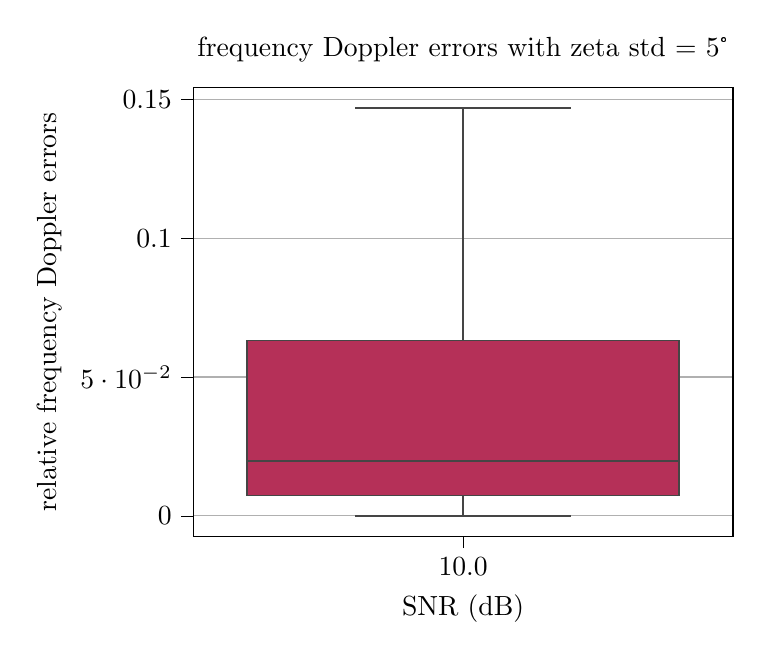
\begin{tikzpicture}

\definecolor{brown1814888}{RGB}{181,48,88}
\definecolor{darkgray176}{RGB}{176,176,176}
\definecolor{darkslategray69}{RGB}{69,69,69}

\begin{axis}[
tick align=outside,
tick pos=left,
title={frequency Doppler errors with zeta std = 5°},
x grid style={darkgray176},
xlabel={SNR (dB)},
xmin=-0.5, xmax=0.5,
xtick style={color=black},
xtick={0},
xticklabels={10.0},
y grid style={darkgray176},
ylabel={relative frequency Doppler errors},
ymajorgrids,
ymin=-0.00733433955362021, ymax=0.154097908171883,
ytick style={color=black}
]
\path [draw=darkslategray69, fill=brown1814888, semithick]
(axis cs:-0.4,0.00732083216923094)
--(axis cs:0.4,0.00732083216923094)
--(axis cs:0.4,0.0631495965464757)
--(axis cs:-0.4,0.0631495965464757)
--(axis cs:-0.4,0.00732083216923094)
--cycle;
\addplot [semithick, darkslategray69]
table {%
0 0.00732083216923094
0 3.4898884481098e-06
};
\addplot [semithick, darkslategray69]
table {%
0 0.0631495965464757
0 0.146760078729814
};
\addplot [semithick, darkslategray69]
table {%
-0.2 3.4898884481098e-06
0.2 3.4898884481098e-06
};
\addplot [semithick, darkslategray69]
table {%
-0.2 0.146760078729814
0.2 0.146760078729814
};
\addplot [semithick, darkslategray69]
table {%
-0.4 0.0196350752402833
0.4 0.0196350752402833
};
\end{axis}

\end{tikzpicture}
